%%%%%%%%%%%%%%%%%%%%%%%%%%%%%%%%%%%%%%%%%%%%%%%%%%%%%%%%%%%%%%%%%%%%%%%%%%%%%%%%%%%%%%%%%%%%%%%%%%%%%
% This template is distributed with ABSOLUTELY NO WARRANTY.
% It serves as a guideline and constitutes a basic structure for a
% thesis/dissertation. The user assumes full responsibility for formatting
% and typesetting their document and for verifying that all the thesis
% requirements set by the University of Tennessee are met. Please refer to the most
% recent UT thesis guide (http://web.utk.edu/~thesis/thesisresources.shtml)
% or contact the thesis consultant (http://web.utk.edu/~thesis/).
% Please report any bugs to the thesis consultant.
%%%%%%%%%%%%%%%%%%%%%%%%%%%%%%%%%%%%%%%%%%%%%%%%%%%%%%%%%%%%%%%%%%%%%%%%%%%%%%%%%%%%%%%%%%%%%%%%%%%%%
% O P T I O N S:
% 1. thesis/dissertation
% 2. monochrome
% 3. all options provided by the report class
\documentclass[dissertation,letterpaper,12pt]{utthesis} 
% Use for two-sided: \documentclass[dissertation,twoside,letterpaper,12pt]{utthesis}

% thesis, one side
% some alternatives are:
%\documentclass[thesis,monochrome,letterpaper,12pt]{utthesis} %thesis, one side, monochrome text
%\documentclass[thesis,twoside,letterpaper,12pt]{utthesis} % thesis, two side
%\documentclass[thesis,monochrome,twoside,letterpaper,12pt]{utthesis} % thesis, two side, monochrome text
% for a dissertation, replace the thesis option by dissertation:
% \documentclass[dissertation,letterpaper,12pt]{utthesis} . . .
\renewcommand{\baselinestretch}{1.5} 	 % line Spacing
%%%%%%%%%%%%%%%%%%%%%%%%%%%%%%%%%%%%%%%%%%%%%%%%%%%%%%%%%%%%%%%%%%%%%%%%%%%%%%%%%%%%%%%%%%%%%%%%%%%%%
% TO DO: FILL IN YOUR INFORMATION BELOW - READ THIS SECTION CAREFULLY
%%%%%%%%%%%%%%%%%%%%%%%%%%%%%%%%%%%%%%%%%%%%%%%%%%%%%%%%%%%%%%%%%%%%%%%%%%%%%%%%%%%%%%%%%%%%%%%%%%%%%
\title{Political Science: Making Dissertations Great Again}	       % title of thesis/dissertation
\author{First Middle Last}                % author's name
\copyrightYear{Year}            % copyright year of your thesis/dissertation
\graduationMonth{Graduation Month}           % month of graduation of your thesis/dissertation
\majorProfessor{Major Prpfessor}	    % advisor's name
\keywords{Political science}	% keywords (optional) separated by commas - these are used in the PDF file properties
\viceProvost{Dixie L. Thompson} % vice provost name
\major{Political Science}	% major: Mechanical Engineering, Aerospace Engineering, Mathematics...
\degree{Doctor of Philosophy}	    % degree: Doctor of Philosophy, Master of Science, Master of Engineering...
\college{Arts \& Sciences}           % college
\dept{Political Science}	% department
\university{The University  of Tennessee, Knoxville}	% school name
% THIS TEMPLATE ACCOMMODATES UP TO 5 COMMITTEE MEMBERS - ENTER ONLY THE NAMES OF THE MEMBERS ON YOUR COMMITTEE
\numberOfCommitteeMembers{3} % enter the number of committee members
\committeeMemberA {Committee Member 1}	% name of first committee member
\committeeMemberB {Committee Member 2}	% name of second committee member
\committeeMemberC {Committee Member 3}	% ... you get the trend!
\committeeMemberD {Committee Member 4}	% if your committee has less than 4 members, you do not need to edit the
\committeeMemberE {Committee Member 5}  % rest of committee names
%%%%%%%%%%%%%%%%%%%%%%%%%%%%%%%%%%%%%%%%%%%%%%%%%%%%%%%%%%%%%%%%%%%%%%%%%%%%%%%%%%%%%%%%%%%%%%%%%%%%%
% LOAD SOME USEFUL PACKAGES
%%%%%%%%%%%%%%%%%%%%%%%%%%%%%%%%%%%%%%%%%%%%%%%%%%%%%%%%%%%%%%%%%%%%%%%%%%%%%%%%%%%%%%%%%%%%%%%%%%%%%
\usepackage{nomencl}                    % produces a nomenclature
\usepackage{float}                      % figure floats
\usepackage{natbib}                     % this package allows you to link your references
\usepackage{graphicx}					% graphics package
\graphicspath{{figures/}{figures/ch3/}{figures/ch4/}}% specify the path where figures are located
\usepackage{fancyhdr}                   % fancy headers and footers
\usepackage{url}                        % nicely format url breaks
\usepackage[inactive]{srcltx}		 	% necessary to use forward and inverse searching in DVI
\usepackage{relsize}                    % font sizing hierarchy
\usepackage{booktabs}                   % professional looking tables
\usepackage[config, labelfont={bf}]{caption,subfig} % nice sub figures
\usepackage{mathrsfs}                   % additional math scripts
\usepackage{tabularx}					%Added for tables - CJA
\usepackage{multirow} 					%Added for itemized lists - CJA
\usepackage{tikz}						%Added for models/figures - CJA
\usetikzlibrary{shapes,arrows}
%%% PACKAGES THAT ARE PRELOADED WITH THE CLASS ARE: amsmath,amsthm,amssymb,setspace,geometry,hyperref,and color
%%%%%%%%%%%%%%%%%%%%%%%%%%%%%%%%%%%%%%%%%%%%%%%%%%%%%%%%%%%%%%%%%%%%%%%%%%%%%%%%%%%%%%%%%%%%%%%%%%%%%
\begin{document}
    \pagenumbering{alph} % this is needed to clear certain issues with the hyperref package
    %
    %\makeApprovalPage % make the approval page - this is the page that needs to be signed & returned to the thesis/dissertation consultant
    %\makeETDApprovalPage % make the Electronic Thesis & Dissertation page - this page is kept with the electronic copy
    % The new approval page is available on the Graduate School's website (http://gradschool.utk.edu/documents/2016/02/thesisdissertation-approval.pdf -- as of August 2017). And, the ETD approval page is now generated by TRACE, and no longer necessary to include in your submission. 
    \addToPDFBookmarks{0}{Front Matter}{rootNode} % create a root node named "Front Matter" in the pdf bookmarks
    \addToPDFBookmarks{1}{Title}{a} % add a pdf bookmark to the title page
    \makeTitlePage % make the title page. Make sure you properly set the \docType
    %
    \pagenumbering{roman}
    \setcounter{page}{2}
    %
    \makeCopyrightPage % make the copyright page
    %
    \addToPDFBookmarks{1}{Dedication}{b} % add a pdf bookmark to the dedication page
    \chapter*{}
\begin{center}
{\centering \it Dedication...}
\end{center}  % include the dedication
    %
    \addToPDFBookmarks{1}{Acknowledgements}{c} % add a pdf bookmark to the acknowledgements page
    \include{front-matter/acknowledgements} % include the acknowledgements
    %
    \addToPDFBookmarks{1}{Quote}{d} % add a pdf bookmark to the quotation page
    \include{front-matter/quote} % include a quote
    %
    \addToPDFBookmarks{1}{Abstract}{e} % add a pdf bookmark to the abstract page
    \chapter*{Abstract}

Lorem ipsum dolor sit amet, consectetur adipiscing elit. Vestibulum ornare fringilla leo sit amet vulputate. Phasellus laoreet libero ut finibus blandit. Pellentesque vel risus sit amet orci vestibulum ultricies. Quisque rhoncus neque lorem, vel commodo ex cursus id. Aenean tristique lectus id ex blandit ultrices. Suspendisse ac arcu pharetra, viverra erat sit amet, iaculis metus. Sed accumsan consequat vehicula. Suspendisse euismod iaculis auctor. Pellentesque malesuada lectus justo, sed feugiat mauris laoreet in. Fusce lacus lacus, cursus vel tristique ac, tincidunt ut neque. In rhoncus odio risus, iaculis dictum diam porttitor non.

Cras eget sagittis libero. Cras egestas, nisi eget rhoncus efficitur, neque diam pretium risus, feugiat aliquet elit elit in lorem. Quisque ex arcu, maximus nec ligula ut, ultrices aliquam sapien. Nulla nunc ex, ornare ut nunc quis, lacinia vehicula risus. Nunc varius elit mauris, et blandit tellus blandit vitae. Vivamus finibus, orci vitae consequat viverra, lorem leo pellentesque nisl, sit amet suscipit arcu dui vel odio. Vestibulum ante ipsum primis in faucibus orci luctus et ultrices posuere cubilia Curae;

Suspendisse potenti. Quisque a porta ante. Nam lacinia semper mi, id dictum augue. Aenean pellentesque, ipsum sit amet vestibulum laoreet, quam purus condimentum purus, in scelerisque ante orci vel urna. In nec congue libero. Aenean tempus, turpis et pharetra luctus, lacus leo blandit odio, sed ullamcorper orci risus in quam. Suspendisse semper aliquet nunc, ac rhoncus massa porttitor eget.  % your abstract
    %
    \renewcommand{\contentsname}{Table of Contents}
    \addToPDFBookmarks{0}{Table of Contents}{f}
    \tableofcontents % generate a table of contents
    %
    %\addToTOC{List of Tables} % this will add the list of tables to the Table of Contents (TOC) -- Removed, CJA
    \listoftables % generate a list of tables
    %
    %\addToTOC{List of Figures} % this will add the list of figures to the Table of Contents (TOC) -- Removed, CJA
    \listoffigures % generate a list of figures
    %
    %\makenomenclature % OPTIONAL
    %\addToPDFBookmarks{0}{Nomenclature}{g} % OPTIONAL
    %\printnomenclature[1.25in] % OPTIONAL
    %
    \newpage
    \pagenumbering{arabic}
    \setcounter{page}{1}
    %%%%%%%%%%%%%%%%%%%%%%%%%%%%%%%%%%%%%%%%%%%%%%%%%%%%%%%%%%%%%%%%%%%%%%%%%%%%%%%%%%%%%%%%%%%%%%%%%%%%%
    % INCLUDE THE CHAPTERS STARTING WITH THE NOMENCLATURE IF PRESENT
    %%%%%%%%%%%%%%%%%%%%%%%%%%%%%%%%%%%%%%%%%%%%%%%%%%%%%%%%%%%%%%%%%%%%%%%%%%%%%%%%%%%%%%%%%%%%%%%%%%%%%
    \include{front-matter/nomenclature} % OPTIONAL
    \chapter{Introduction} \label{ch:intro}

Most of the settings are the same as those provided in the original dissertation template, created by Tony Saad, with a few changes to reflect the  \href{http://gradschool.utk.edu/thesesdissertations/}{updated formatting requirements}. These changes are (in no particular order):

 \begin{itemize} 
 	\item A new \textit{hypothesis} environment, in addition to the \textit{theorem, correlary,} and \textit{lemma} environments. For example: \hyperref[hyp:3a]{Hypothesis \ref{hyp:3a}} and \ref{hyp:3b}. 
 	\item Margins were changed to the following:
	 	\begin{itemize} \setlength{\itemsep}{0pt} 
	 		\item[] \begin{verbatim}
			 		left = 1.25in,
			 		right = 1.25in,
			 		top = 1.0in,
			 		bottom = 1.375in
			 		\end{verbatim} \vspace*{-2em}
	 	\end{itemize}
	 \item 	Several packages were added, such as \href{https://www.ctan.org/pkg/longtable?lang=en}{\textsf{longtable}},  \href{https://www.ctan.org/pkg/multirow}{\textsf{multirow}}, \href{https://www.ctan.org/pkg/tabularx}{\textsf{tabularx}}, and \href{https://www.ctan.org/pkg/pgf}{\textsf{TikZ/pgf}}. 
	 \item Note the file path for figures. I grouped them by chapter (e.g. `ch3' \& `ch4'):
		 \begin{itemize}
		 	\item[] \begin{verbatim}
		 	\graphicspath{{figures/}{figures/ch3/}{figures/ch4/}}
		 	\end{verbatim} \vspace*{-2em}
		 \end{itemize}
 	\item Additionally, there were a few stylistic changes, such as changing `Contents' to `Table of Contents,' adding Appendices to the Table of Contents, moving the Bibliography title to its own page, and changes to the color of links, references, etc. 
 	\item Other considerations/changes to make:
	 	\begin{itemize} 
	 		\item If you have tables/figures you want to turn sideways, \href{https://www.ctan.org/pkg/landscape?lang=en}{\textsf{landscape}} environment provides this, but you must manually rotate each page using Adobe (or other PDF editor) after you compile the document. 
	 		\item If you need to use \href{https://www.ctan.org/pkg/longtable?lang=en}{\textsf{longtable}} environment the , you will need to include a `first header' and `second header' that includes the table name, number, and ``\textit{Continued from previous page}'' (e.g. \hyperref[longtable]{Table \ref{longtable}}). 
	 		\item ``Table'' and ``Figure'' labels need to go above and below the table and figure, respectively (e.g. \hyperref[table]{Table \ref{table}} \& \hyperref[figure]{Figure \ref{figure}}). 
	 		\item Tables were made using \href{https://cran.r-project.org/web/packages/stargazer/vignettes/stargazer.pdf}{\textsf{stargazer}} in R \citep{stargazer}.
	 	\end{itemize}
 \end{itemize}

    \chapter{The Second Chapter} \label{ch:2}


Lorem ipsum dolor sit amet, consectetur adipiscing elit. Nulla scelerisque turpis dui, id dictum ipsum semper non. In sollicitudin odio dui, nec fermentum sem congue et. Nulla vitae ante ut nisl lobortis tempor. In sed elit nisl. Donec blandit in ligula venenatis lobortis. Etiam nunc mauris, auctor finibus imperdiet at, bibendum egestas nulla. Aliquam sed aliquet leo, vitae ornare urna. Ut eu porttitor tortor. Suspendisse dapibus mi risus, egestas egestas odio commodo eget. Fusce orci orci, ultricies nec tempus sit amet, eleifend lacinia elit. Morbi ut ante viverra, cursus dolor tempus, semper lacus. Quisque bibendum hendrerit ullamcorper. Mauris risus ante, auctor eget leo non, faucibus blandit nisi. Aliquam lobortis, ante id egestas ullamcorper, ligula felis accumsan mauris, vel bibendum neque libero ac erat. Maecenas dictum velit nulla, non molestie lorem consectetur sit amet. 

\begin{hyp} \label{hyp:3a}
	This thing will happen.
\end{hyp}

\begin{hyp} \label{hyp:3b}
	This other thing will happen.
\end{hyp} 	


Curabitur porttitor nulla at blandit euismod. Nunc sit amet dapibus leo, quis accumsan sapien. Nulla ut mattis tortor, vitae euismod quam. Cras turpis velit, pretium vitae feugiat at, malesuada vel nunc. Proin sed pellentesque odio. Praesent maximus, nunc ac finibus pretium, turpis lectus hendrerit neque, eget semper orci nisi ut sapien. Nam semper cursus orci ut condimentum. 

\begin{landscape} 
	\vspace*{\fill}
	\thispagestyle{empty}
	\begin{table}[!htbp] \centering 
		\caption{The Best Results} 
		\label{table} 
		\begin{tabular}{@{\extracolsep{2pt}}lccc} 
			\\[-1.8ex]\hline 
			\hline \\[-1.8ex] 
			& \multicolumn{3}{c}{\textit{Dependent variable:}} \\ 
			\cline{2-4} 
			\\[-1.8ex] & \multicolumn{3}{c}{Winning} \\ 
			\\[-1.8ex] & (Model 1) & (Model 2) & (Model 3)\\ 
			\hline \\[-1.8ex] 
			Variable 1 & 0.10$^{**}$ & 0.20$^{***}$ & 0.30$^{***}$ \\ 
			& (0.01) & (0.01) & (0.01) \\
			Variable 2 & 0.10$^{**}$ & 0.20$^{***}$ & 0.30$^{***}$ \\  
			& (0.01) & (0.01) & (0.01) \\
			Variable 3 & 0.10$^{**}$ & 0.20$^{***}$ & 0.30$^{***}$ \\  
			& (0.01) & (0.01) & (0.01) \\ 
			Constant & 1.00$^{***}$ & 1.25$^{***}$ & 01.50$^{***}$ \\ 
			& (0.08) & (0.06) & (0.13) \\ 
			\hline \\[-1.8ex] 
			Observations & 500 & 500 & 500 \\ 
			R$^{2}$ & 0.45 & 0.50 & 0.55 \\ 
			Adjusted R$^{2}$ & 0.40 & 0.45 & 0.50 \\ 
			Residual Std. Error & 0.00 (df = 000) & 0.00 (df = 000) & 0.00 (df = 000) \\ 
			F Statistic & 10.00$^{***}$ (df = 0; 000) & 10.00$^{***}$ (df = 0; 000) & 10.00$^{***}$ (df = 0; 000) \\ 
			\hline 
			\hline \\[-1.8ex] 
			\textit{Note:}  & \multicolumn{3}{r}{$^{*}$p$<$0.1; $^{**}$p$<$0.05; $^{***}$p$<$0.01} \\ 
		\end{tabular} 
	\end{table}
	\vfill
	\raisebox{-.5in}{\makebox[\linewidth]{\thepage}}
\end{landscape}	

    \chapter{The Third Chapter} \label{ch:3}

Lorem ipsum dolor sit amet, consectetur adipiscing elit. Mauris fermentum convallis pulvinar. Pellentesque luctus elit eu cursus luctus. Mauris mi mauris, dapibus non eros ac, vulputate facilisis nibh. Aenean et mattis mauris. Proin lacus risus, elementum quis tortor at, venenatis vulputate massa. Nunc accumsan, tellus ut molestie rutrum, turpis lorem tristique diam, at euismod turpis erat a felis. Morbi nec ornare diam.

Cras efficitur diam neque, sed congue sem sagittis sed. Sed venenatis eget ex sit amet pellentesque. Vestibulum et tortor id leo finibus tristique vel ac arcu. Pellentesque habitant morbi tristique senectus et netus et malesuada fames ac turpis egestas. Curabitur tempus in ante non facilisis. In at leo at justo tincidunt pharetra. Nullam rhoncus augue ut aliquam fermentum. Vestibulum sit amet arcu mattis, placerat leo id, placerat mauris. In egestas molestie mollis. Donec cursus neque vitae sapien maximus lobortis. Nunc vel orci a odio laoreet rutrum vitae ut libero. Mauris odio quam, consequat a semper nec, gravida vel sem. Duis sodales consectetur orci, quis dignissim justo dictum id. Ut volutpat magna non ante tempor finibus. Praesent rhoncus tellus sit amet ex suscipit, et imperdiet diam hendrerit. Vestibulum rutrum non orci sit amet ornare. Nullam metus nibh, semper quis.

 \begin{spacing}{1} \def\arraystretch{1.25} % \arraystretch gives some extra space between lines if you need it 
	{\small
 		\begin{longtable}{lcccc}											
 			\caption{Bigly Model Full of Lots \& Lots of Variables} 														
 			\label{longtable} 													
 			\\[-1.8ex]\hline 
 			\hline \\[-2ex]																
 			Variable	&	Model 1	&	Model 2	&	  Model 3	& Model 4 	\\	
 			\hline \\[-1.8ex]
 			\endfirsthead
 			\multicolumn{5}{c}%
 			{\textbf{\tablename\ \thetable} -- \textit{Continued from previous page}} \\
 			\\[-1.8ex]\hline 	
 			Variable	&	Model 1	&	Model 2	&	  Model 3	& Model 4 	\\		
 			\hline \\[-1.8ex]
 			\endhead
 			\hline 
 			\multicolumn{5}{l}{$^{*}$p $<$ .1; $^{**}$p $<$ .05; $^{***}$p $<$ .01}
 			\endfoot
 			This & 0.25$^{***}$ & 0.25$^{***}$ & 0.25$^{***}$ & 0.25$^{***}$ \\
			&	(0.05)	&	(0.05)	&	(0.05)	&	(0.05) \\	 
 			Is & 0.25$^{***}$ & 0.25$^{***}$ & 0.25$^{***}$ & 0.25$^{***}$ \\
 			&	(0.05)	&	(0.05)	&	(0.05)	&	(0.05) \\	 
 			A & 0.25$^{***}$ & 0.25$^{***}$ & 0.25$^{***}$ & 0.25$^{***}$ \\
 			&	(0.05)	&	(0.05)	&	(0.05)	&	(0.05) \\	 
 			Really & 0.25$^{***}$ & 0.25$^{***}$ & 0.25$^{***}$ & 0.25$^{***}$ \\
 			&	(0.05)	&	(0.05)	&	(0.05)	&	(0.05) \\	 
 			Long & 0.25$^{***}$ & 0.25$^{***}$ & 0.25$^{***}$ & 0.25$^{***}$ \\
 			&	(0.05)	&	(0.05)	&	(0.05)	&	(0.05) \\	 
 			Table & 0.25$^{***}$ & 0.25$^{***}$ & 0.25$^{***}$ & 0.25$^{***}$ \\
 			&	(0.05)	&	(0.05)	&	(0.05)	&	(0.05) \\	 
 			Just & 0.25$^{***}$ & 0.25$^{***}$ & 0.25$^{***}$ & 0.25$^{***}$ \\
 			&	(0.05)	&	(0.05)	&	(0.05)	&	(0.05) \\	 
 			In & 0.25$^{***}$ & 0.25$^{***}$ & 0.25$^{***}$ & 0.25$^{***}$ \\
 			&	(0.05)	&	(0.05)	&	(0.05)	&	(0.05) \\	 
 			Case & 0.25$^{***}$ & 0.25$^{***}$ & 0.25$^{***}$ & 0.25$^{***}$ \\
 			&	(0.05)	&	(0.05)	&	(0.05)	&	(0.05) \\	 
 			You & 0.25$^{***}$ & 0.25$^{***}$ & 0.25$^{***}$ & 0.25$^{***}$ \\
 			&	(0.05)	&	(0.05)	&	(0.05)	&	(0.05) \\	 
 			Have & 0.25$^{***}$ & 0.25$^{***}$ & 0.25$^{***}$ & 0.25$^{***}$ \\
 			&	(0.05)	&	(0.05)	&	(0.05)	&	(0.05) \\	 
 			A & 0.25$^{***}$ & 0.25$^{***}$ & 0.25$^{***}$ & 0.25$^{***}$ \\
 			&	(0.05)	&	(0.05)	&	(0.05)	&	(0.05) \\	 
 			Model & 0.25$^{***}$ & 0.25$^{***}$ & 0.25$^{***}$ & 0.25$^{***}$ \\
 			&	(0.05)	&	(0.05)	&	(0.05)	&	(0.05) \\	 
 			With & 0.25$^{***}$ & 0.25$^{***}$ & 0.25$^{***}$ & 0.25$^{***}$ \\
 			&	(0.05)	&	(0.05)	&	(0.05)	&	(0.05) \\	 
 			A & 0.25$^{***}$ & 0.25$^{***}$ & 0.25$^{***}$ & 0.25$^{***}$ \\
 			&	(0.05)	&	(0.05)	&	(0.05)	&	(0.05) \\	 
 			Ton & 0.25$^{***}$ & 0.25$^{***}$ & 0.25$^{***}$ & 0.25$^{***}$ \\
 			&	(0.05)	&	(0.05)	&	(0.05)	&	(0.05) \\	 
 			Of & 0.25$^{***}$ & 0.25$^{***}$ & 0.25$^{***}$ & 0.25$^{***}$ \\
 			&	(0.05)	&	(0.05)	&	(0.05)	&	(0.05) \\	 
 			Variables & 0.25$^{***}$ & 0.25$^{***}$ & 0.25$^{***}$ & 0.25$^{***}$ \\
 			&	(0.05)	&	(0.05)	&	(0.05)	&	(0.05) \\	 
 			Or & 0.25$^{***}$ & 0.25$^{***}$ & 0.25$^{***}$ & 0.25$^{***}$ \\
 			&	(0.05)	&	(0.05)	&	(0.05)	&	(0.05) \\	 
 			Just & 0.25$^{***}$ & 0.25$^{***}$ & 0.25$^{***}$ & 0.25$^{***}$ \\
 			&	(0.05)	&	(0.05)	&	(0.05)	&	(0.05) \\	 
 			Need & 0.25$^{***}$ & 0.25$^{***}$ & 0.25$^{***}$ & 0.25$^{***}$ \\
 			&	(0.05)	&	(0.05)	&	(0.05)	&	(0.05) \\	 	
 			To & 0.25$^{***}$ & 0.25$^{***}$ & 0.25$^{***}$ & 0.25$^{***}$ \\
 			&	(0.05)	&	(0.05)	&	(0.05)	&	(0.05) \\	 	
 			List & 0.25$^{***}$ & 0.25$^{***}$ & 0.25$^{***}$ & 0.25$^{***}$ \\
 			&	(0.05)	&	(0.05)	&	(0.05)	&	(0.05) \\	 	
 			A & 0.25$^{***}$ & 0.25$^{***}$ & 0.25$^{***}$ & 0.25$^{***}$ \\
 			&	(0.05)	&	(0.05)	&	(0.05)	&	(0.05) \\	 
 			Bunch & 0.25$^{***}$ & 0.25$^{***}$ & 0.25$^{***}$ & 0.25$^{***}$ \\
 			&	(0.05)	&	(0.05)	&	(0.05)	&	(0.05) \\	 
 			Of & 0.25$^{***}$ & 0.25$^{***}$ & 0.25$^{***}$ & 0.25$^{***}$ \\
 			&	(0.05)	&	(0.05)	&	(0.05)	&	(0.05) \\	 	 
 			Things & 0.25$^{***}$ & 0.25$^{***}$ & 0.25$^{***}$ & 0.25$^{***}$ \\
 			&	(0.05)	&	(0.05)	&	(0.05)	&	(0.05) \\	 								
 		\end{longtable}}
  \end{spacing} 
 	

    \chapter{The Fourth Chapter} \label{ch:4}

Lorem ipsum dolor sit amet, consectetur adipiscing elit. Morbi tincidunt quam erat, sit amet lacinia tellus maximus ac. Aliquam lobortis justo et est scelerisque, eget scelerisque magna commodo. In nibh odio, egestas quis pretium at, fermentum a dui. Fusce quis porta arcu. Lorem ipsum dolor sit amet, consectetur adipiscing elit. Pellentesque ornare magna arcu, feugiat ornare nulla pharetra at. Nam nec velit urna. Cras vitae diam nec augue congue ullamcorper sit amet eu mi. Sed at lacinia nunc. Integer vehicula maximus arcu, blandit volutpat lorem pellentesque quis. Sed a maximus nisl, mollis mattis nunc. Suspendisse varius cursus dapibus.

Curabitur iaculis euismod sem, vel lobortis felis. Proin vitae rhoncus velit, in vestibulum nisi. Etiam sed metus nec dui ullamcorper suscipit. Donec rhoncus, mauris vel sollicitudin suscipit, sem magna efficitur est, ac iaculis eros enim id nisl. Morbi sollicitudin justo eu fermentum euismod. Donec quis nibh et arcu ultricies vehicula ut vel lectus. Praesent vulputate arcu vel commodo efficitur. Integer sagittis arcu id nisl dictum aliquam. Phasellus imperdiet consequat condimentum. Aliquam in scelerisque nulla. Donec consequat dolor in nisl vestibulum, eget faucibus dui interdum.


\begin{landscape} 
	\thispagestyle{empty}
	%\vspace*{\fill}
	\begin{figure}[!htbp] 
		\centering
		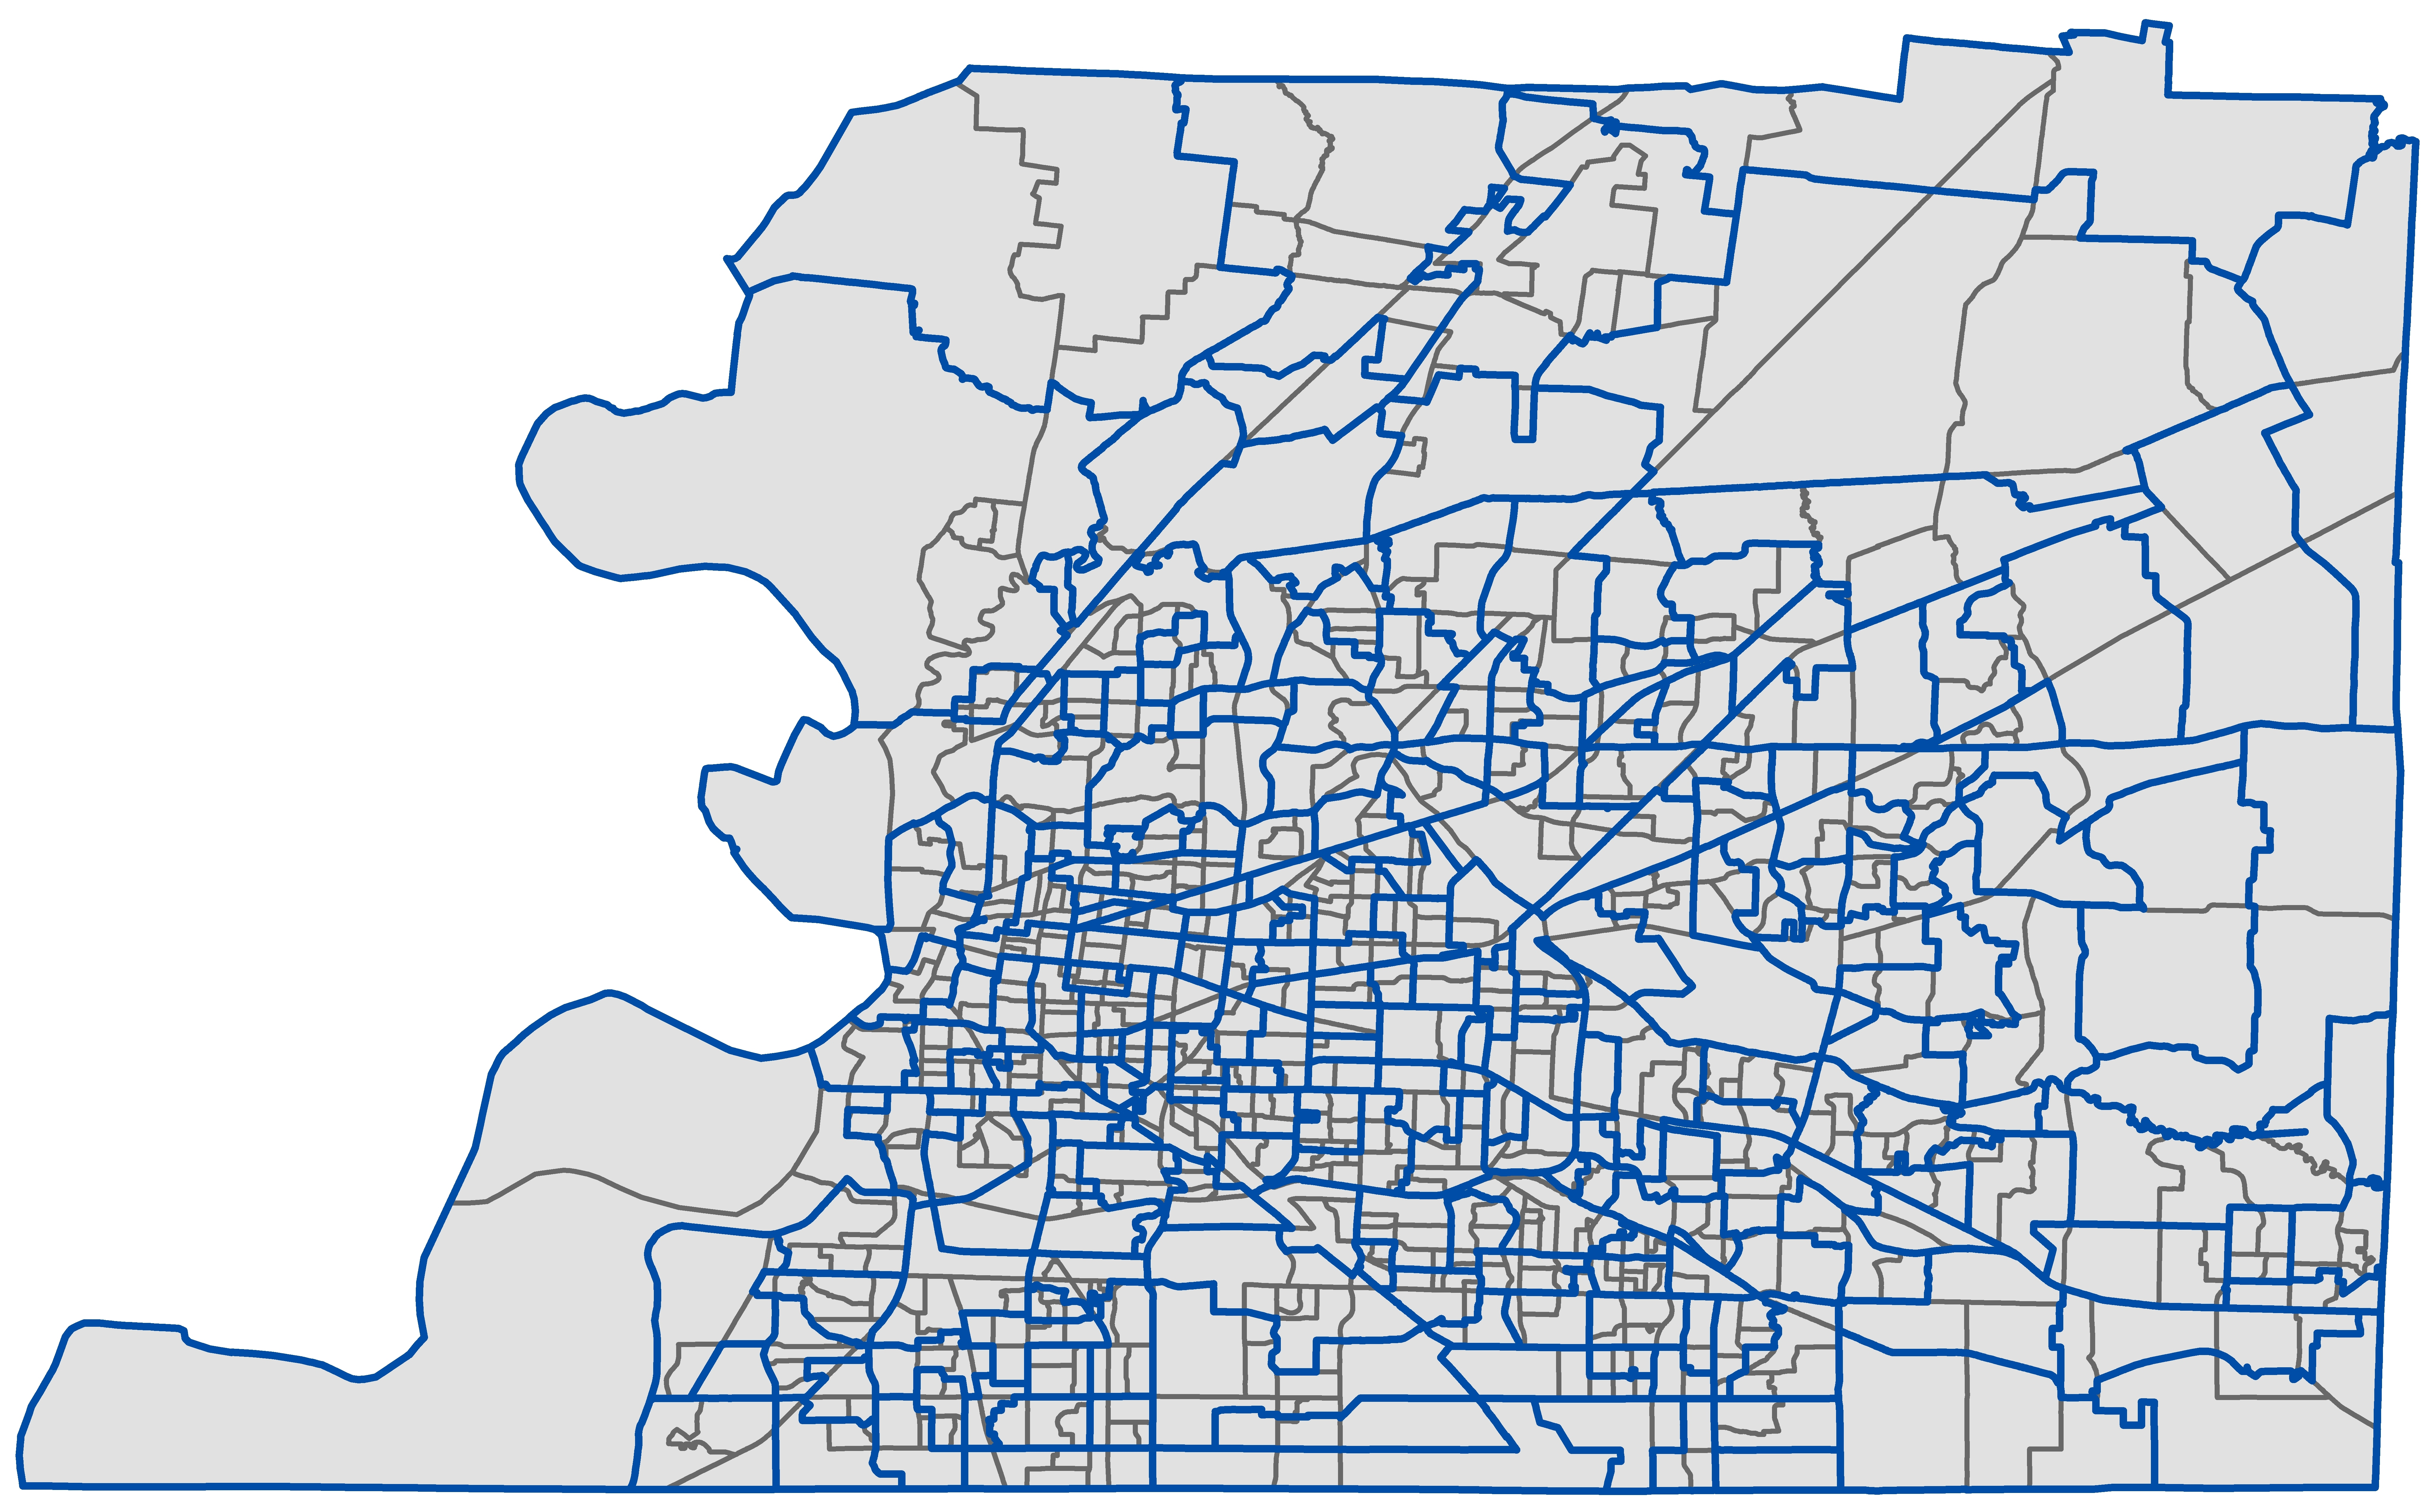
\includegraphics{ShelbyCo} 
		\caption{Shelby County Census Blocks, With Precint Overlay}
		\label{figure}
	\end{figure}
	%\vfill
	\raisebox{-.5in}{\makebox[\linewidth]{\thepage}}
\end{landscape}




    \chapter{Conclusions} \label{ch:5}

Lorem ipsum dolor sit amet, consectetur adipiscing elit. Praesent ac sodales est. Aenean non consequat risus. Suspendisse a enim in leo convallis accumsan sit amet ac justo. Ut rhoncus, mauris eget malesuada semper, neque neque feugiat neque, sit amet finibus ante elit et lacus. Curabitur tincidunt tellus felis, eget eleifend erat imperdiet sed. In congue magna ac felis consequat, sed mollis magna fermentum. Curabitur ornare ut lectus sodales euismod. Phasellus posuere, mi eget suscipit accumsan, nunc ipsum posuere ante, sit amet efficitur ligula risus nec risus. Maecenas finibus in purus in convallis. Etiam tempus aliquet ligula vel faucibus. Maecenas accumsan sapien in lacus scelerisque, non mollis neque auctor. Sed et rhoncus lectus. Morbi bibendum sapien quis efficitur dignissim. Curabitur tristique augue eget elit ornare, eget condimentum leo venenatis. Morbi porta dapibus sodales.

Sed laoreet diam id lacus consectetur, quis pellentesque mauris tempor. Donec venenatis blandit dolor, sit amet varius est efficitur vitae. Quisque rutrum magna sit amet purus efficitur, et viverra dui efficitur. Vestibulum mattis vehicula elit, ac blandit odio pellentesque quis. Integer ac justo eu diam eleifend fermentum quis vitae magna. Duis efficitur ac leo ut facilisis. Ut et lacinia leo. Cras est sem, convallis a rutrum nec, semper sed ipsum. Aliquam orci nulla, dictum et cursus id, viverra id est. Phasellus aliquet lectus ac leo molestie, eu volutpat nibh malesuada. 
    %%%%%%%%%%%%%%%%%%%%%%%%%%%%%%%%%%%%%%%%%%%%%%%%%%%%%%%%%%%%%%%%%%%%%%%%%%%%%%%%%%%%%%%%%%%%%%%%%%%%%
    % BIBLIOGRAPHY
    %%%%%%%%%%%%%%%%%%%%%%%%%%%%%%%%%%%%%%%%%%%%%%%%%%%%%%%%%%%%%%%%%%%%%%%%%%%%%%%%%%%%%%%%%%%%%%%%%%%%%
    \makeBibliographyPage % make the bibliography title page - can be edited in ut-thesis-template.tex
    \bibliographystyle{apalike} % bibliography style - recommend using apalike-doi as it hyperlinks DOIs
    \renewcommand{\bibname}{\vspace*{-1.5in}} % Remove ``Bibliography'' from top of page and shift references up -- CJA 
    \bibliography{references/references-dissertation} % references.bib included in the references directory
    %%%%%%%%%%%%%%%%%%%%%%%%%%%%%%%%%%%%%%%%%%%%%%%%%%%%%%%%%%%%%%%%%%%%%%%%%%%%%%%%%%%%%%%%%%%%%%%%%%%%%
    % APPENDIX - OPTIONAL - COMMENT IF NOT NEEDED
    %%%%%%%%%%%%%%%%%%%%%%%%%%%%%%%%%%%%%%%%%%%%%%%%%%%%%%%%%%%%%%%%%%%%%%%%%%%%%%%%%%%%%%%%%%%%%%%%%%%%%
    \makeAppendixPage   % make the appendix title page - can be edited in ut-thesis-template.tex \addToTOC{List of Figures}
    \appendix
    \chapter{An Example Model} 

% Define block styles

\tikzstyle{decision} = [diamond, draw, fill=blue!20, 
text width=4.5em, text badly centered, node distance=3cm, inner sep=0pt]
\tikzstyle{block} = [rectangle, draw, fill=blue!20, 
text width=11em, text centered, rounded corners, minimum height=4em]
\tikzstyle{line} = [draw, -latex']
\tikzstyle{cloud} = [draw, ellipse,fill=blue!20, node distance=3cm,
minimum height=2em]
\begin{figure}[!htbp] %\hspace*{-.75cm}
	\label{model} 
	\begin{tikzpicture}[node distance = 1cm, >=latex', font={\footnotesize}]
	% Place nodes
	\node [block] (institution) {Institutional Context ($V_1$)};
	\node [block, below right of=institution, node distance=4cm] (emergence) {Unified Elites ($V_2$):
		\begin{itemize}
		\item[--] Text
		\end{itemize}};
	\node [block, below left of=institution, node distance=4cm] (divided) {Elites Divided ($V_2$): 
		\begin{itemize}
		\item[--] Text
		\end{itemize}};
	\node [block, below of=emergence, node distance=4cm] (commission) {Creation of Commission ($V_3-V_8$):
		\begin{itemize}
		\item[--] Text ($V_3-V_8$)
		\end{itemize}};
	\node [block, below of=commission, below of=emergence, node distance=5cm] (strong) {Strong Campaign ($V_9$):
		\begin{itemize}
		\item[--] Text
		\end{itemize}};
	\node [block, left of=anti, below of=divided, node distance=4cm] (weak) {Weak Campaign ($V_9$):
		\begin{itemize}
		\item[--] Text
		\end{itemize}};
	\node [block, below of=divided, node distance=10cm] (anti) {Opposition Campaign ($V_{10}$):
		\begin{itemize}
		\item[--] Text
		\end{itemize}};
	\node [decision, below of=strong, node distance=4cm] (success) {Outcome 2};
	\node [cloud, below of=anti, node distance=4cm] (fail) {Outcome 1};
	%\node [cloud, below of=decide, node distance=3cm] (stop) {stop};
	% Draw edges
	\path [line] (institution) -- (emergence);
	\path [line, dashed] (institution) -- (divided);
	\path [line] (emergence) -- (commission);
	\path [line] (commission) -- (strong);
	\path [line, dashed] (commission) -- (weak);
	\path [line, dashed] (commission) -- (anti);
	%\path [line] (decide) -| node [near start] {yes} (update);
	%\path [line] (update) |- (identify);
	%\path [line] (decide) -- node {no}(stop);
	\path [line,dashed] (weak) |- (fail);
	\path [line,dashed] (divided) -- (anti);
	\path [line,dashed] (anti) -- (fail);
	\path [line] (strong) -- (success);
	\end{tikzpicture}
	\caption{An Example \href{https://www.ctan.org/pkg/pgf}{\textsf{TikZ/pgf}} Model}
\end{figure}
    \chapter{Additional Information }  

Additional information here.
    %\include{back-matter/appendix-3}
    %%%%%%%%%%%%%%%%%%%%%%%%%%%%%%%%%%%%%%%%%%%%%%%%%%%%%%%%%%%%%%%%%%%%%%%%%%%%%%%%%%%%%%%%%%%%%%%%%%%%%
    % A VITA IS REQUIRED
    %%%%%%%%%%%%%%%%%%%%%%%%%%%%%%%%%%%%%%%%%%%%%%%%%%%%%%%%%%%%%%%%%%%%%%%%%%%%%%%%%%%%%%%%%%%%%%%%%%%%%
    \addToTOC{Vita}
    \chapter*{Vita} 

Vita goes here...
\end{document}
